%%%%%%%%%%%%%%%%%%%%%%%%%%%%%%%%%%%%%%%%%
% Beamer Presentation
% LaTeX Template
% Version 1.0 (10/11/12)
%
% This template has been downloaded from:
% http://www.LaTeXTemplates.com
%
% License:
% CC BY-NC-SA 3.0 (http://creativecommons.org/licenses/by-nc-sa/3.0/)
%
%%%%%%%%%%%%%%%%%%%%%%%%%%%%%%%%%%%%%%%%%

%----------------------------------------------------------------------------------------
%	PACKAGES AND THEMES
%----------------------------------------------------------------------------------------

\documentclass{beamer}
\mode<presentation> {

% The Beamer class comes with a number of default slide themes
% which change the colors and layouts of slides. Below this is a list
% of all the themes, uncomment each in turn to see what they look like.

%\usetheme{default}
%\usetheme{AnnArbor}
%\usetheme{Antibes}
%\usetheme{Bergen}
%\usetheme{Berkeley}
%\usetheme{Berlin}
%\usetheme{Boadilla}
%\usetheme{CambridgeUS}
%\usetheme{Copenhagen}
%\usetheme{Darmstadt}
%\usetheme{Dresden}
%\usetheme{Frankfurt}
%\usetheme{Goettingen}
%\usetheme{Hannover}
%\usetheme{Ilmenau}
%\usetheme{JuanLesPins}
%\usetheme{Luebeck}
\usetheme{Madrid}
%\usetheme{Malmoe}
%\usetheme{Marburg}
%\usetheme{Montpellier}
%\usetheme{PaloAlto}
%\usetheme{Pittsburgh}
%\usetheme{Rochester}
%\usetheme{Singapore}
%\usetheme{Szeged}
%\usetheme{Warsaw}

% As well as themes, the Beamer class has a number of color themes
% for any slide theme. Uncomment each of these in turn to see how it
% changes the colors of your current slide theme.

%\usecolortheme{albatross}
%\usecolortheme{beaver}
%\usecolortheme{beetle}
%\usecolortheme{crane}
%\usecolortheme{dolphin}
%\usecolortheme{dove}
%\usecolortheme{fly}
%\usecolortheme{lily}
%\usecolortheme{orchid}
%\usecolortheme{rose}
%\usecolortheme{seagull}
%\usecolortheme{seahorse}
%\usecolortheme{whale}
%\usecolortheme{wolverine}

%\setbeamertemplate{footline} % To remove the footer line in all slides uncomment this line
%\setbeamertemplate{footline}[page number] % To replace the footer line in all slides with a simple slide count uncomment this line

%\setbeamertemplate{navigation symbols}{} % To remove the navigation symbols from the bottom of all slides uncomment this line
}
\definecolor{TsinghuaPurple}{RGB}{128,0,128}
\setbeamercolor{frametitle}{bg=TsinghuaPurple}
\setbeamercolor{section in head/foot}{bg=TsinghuaPurple}
\setbeamercolor{author in head/foot}{bg=TsinghuaPurple}
\setbeamercolor{date in head/foot}{bg=TsinghuaPurple}
\setbeamercolor{palette primary}{bg=TsinghuaPurple}
\setbeamercolor{palette secondary}{bg=TsinghuaPurple}
\setbeamercolor{block title}{bg=TsinghuaPurple}
%\setbeamercolor{palette tertiary}{fg=black, bg=gold}
%\definecolor{gold}{HTML}{FDD017}
%\definecolor{deep sky blue}{HTML}{3BB9FF}
%\definecolor{light sky blue}{HTML}{82CAFA}
%\definecolor{mybackground}{HTML}{82CAFA}
%\definecolor{myforeground}{HTML}{0000A0}
%\setbeamercolor{normal text}{fg=black,bg=white}
%\setbeamercolor{alerted text}{fg=red}
%\setbeamercolor{example text}{fg=black}
%\setbeamercolor{background canvas}{fg=myforeground, bg=white}
%\setbeamercolor{background}{fg=myforeground, bg=mybackground}

\usepackage{graphicx} % Allows including images
\usepackage{booktabs} % Allows the use of \toprule, \midrule and \bottomrule in tables

\usepackage{epstopdf} % Allows the use of eps for pdflatex
\usepackage{multirow} % Allows the use of multirow in tabular

%----------------------------------------------------------------------------------------
%	TITLE PAGE
%----------------------------------------------------------------------------------------

\title[Introduction to Modern Database Systems]{	Processing of Probabilistic Skyline Queries Using MapReduce} % The short title appears at the bottom of every slide, the full title is only on the title page

\author{Qingfu Wen} % Your name
\institute[THU] % Your institution as it will appear on the bottom of every slide, may be shorthand to save space
{
School of Software, Tsinghua University\\ % Your institution for the title page
\medskip
\texttt{qingfu.wen@gmail.com} % Your email address
\\
\medskip
\text{Author: Yoonjae Park, Jun-Ki Min, Kyuseok Shim}
}
\date{\today} % Date, can be changed to a custom date

\begin{document}


%--------------Frame 1---------------------
\begin{frame}
\titlepage % Print the title page as the first slide
\begin{figure}[htpb]
  \begin{center}
	
\includegraphics[width=0.18\linewidth]{Tsinghua_University_Logo.eps}
  \end{center}
\end{figure}
\end{frame}

%--------------Frame 2---------------------
%\begin{frame}
%\frametitle{Overview} % Table of contents slide, comment this block out to remove it
%\tableofcontents % Throughout your presentation, if you choose to use \section{} and \subsection{} commands, these will automatically be printed on this slide as an overview of your presentation
%\end{frame}

%----------------------------------------------------------------------------------------
%	PRESENTATION SLIDES
%----------------------------------------------------------------------------------------
%------------------------------------------------
%\section{Introduction} % Sections can be created in order to organize your presentation into discrete blocks, all sections and subsections are automatically printed in the table of contents as an overview of the talk
%------------------------------------------------

%--------------Frame 2---------------------
\begin{frame}
\frametitle{Probabilistic Skylines}
\begin{columns}[t] % The "c" option specifies centered vertical alignment while the "t" option is used for top vertical alignment

\column{.42\textwidth} % Left column and width
\begin{figure}[htpb]
  \begin{center}
	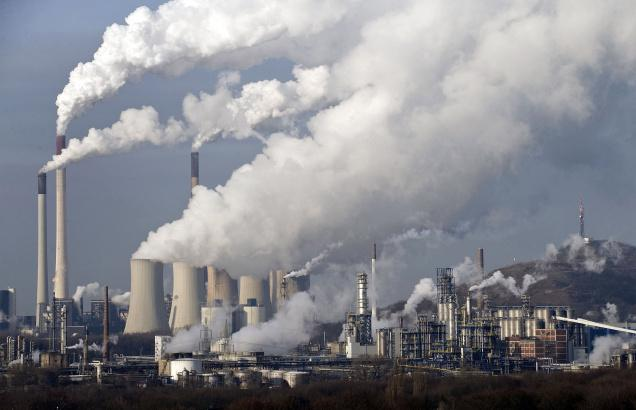
\includegraphics[width=1\linewidth]{pollution.jpg}
  \end{center}
\end{figure}
\begin{figure}[htpb]
  \begin{center}
	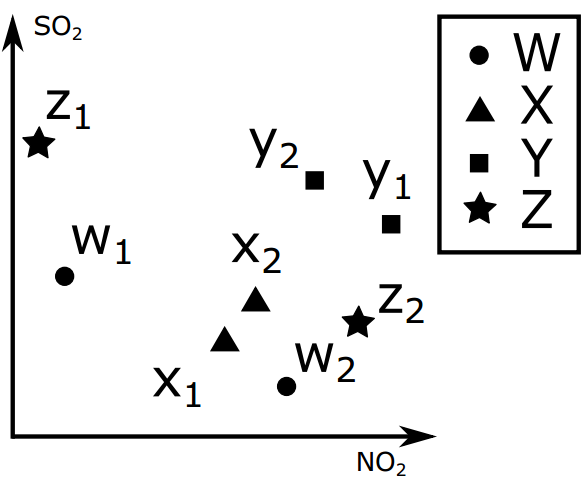
\includegraphics[width=0.75\linewidth]{coordinate.png}
  \end{center}
\end{figure}

\column{.58\textwidth} % Right column and width
\begin{table}[htbp]
\scriptsize
\begin{tabular}{|c|c|c|c|c|}
\hline Object&Instance&NO$_2$&SO$_2$& Probability\\
\hline
\multirow{2}{*}{W}
             &w$_1$   &10    &40    &0.5\\
             &w$_2$   &75    &10    &0.4\\\hline
\multirow{2}{*}{X}
             &x$_1$   &55    &20    &0.2\\
             &x$_2$   &65    &30    &0.2\\\hline
\multirow{2}{*}{Y}
             &y$_1$   &95    &60    &0.8\\
             &y$_2$   &80    &70    &0.2\\\hline
\multirow{2}{*}{Z}
             &z$_1$   & 5    &80    &0.5\\
             &z$_2$   &90    &25    &0.5\\
\hline
\end{tabular}
\end{table}

\end{columns}
\end{frame}

%--------------Frame 3---------------------
\begin{frame}
\frametitle{Probabilistic Skylines}
\begin{columns}[t] % The "c" option specifies centered vertical alignment while the "t" option is used for top vertical alignment

\column{.42\textwidth} % Left column and width
\begin{figure}[htpb]
  \begin{center}
	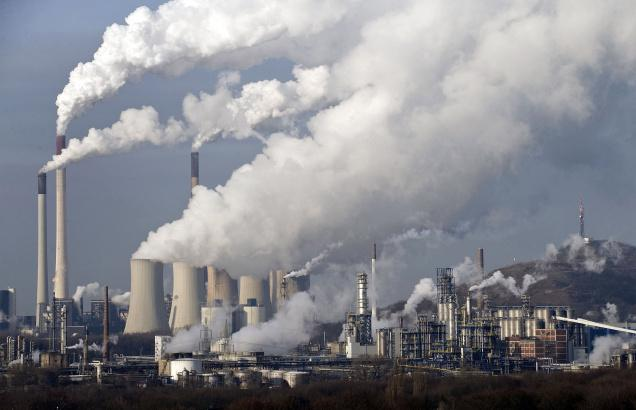
\includegraphics[width=1\linewidth]{pollution.jpg}
  \end{center}
\end{figure}
\begin{figure}[htpb]
  \begin{center}
	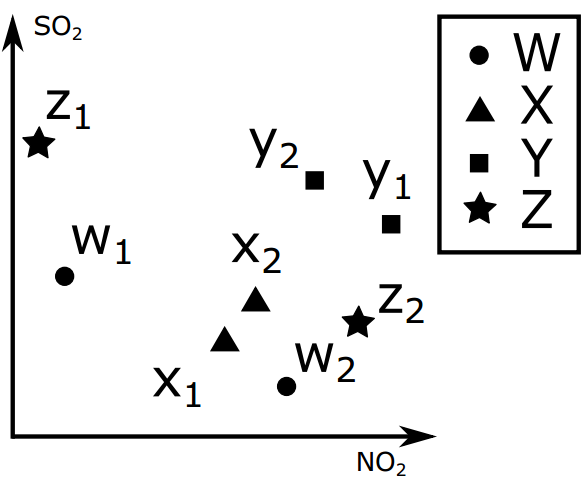
\includegraphics[width=0.75\linewidth]{coordinate.png}
  \end{center}
\end{figure}

\column{.58\textwidth} % Right column and width
\begin{table}[htbp]
\scriptsize
\begin{tabular}{|c|c|c|c|c|}
\hline Object&Instance&NO$_2$&SO$_2$& Probability\\
\hline
\multirow{2}{*}{W}
             &w$_1$   &10    &40    &0.5\\
             &w$_2$   &75    &10    &0.4\\\hline
\multirow{2}{*}{X}
             &x$_1$   &55    &20    &0.2\\
             &x$_2$   &65    &30    &0.2\\\hline
\multirow{2}{*}{Y}
             &y$_1$   &95    &60    &0.8\\
             &y$_2$   &80    &70    &0.2\\\hline
\multirow{2}{*}{Z}
             &z$_1$   & 5    &80    &0.5\\
             &z$_2$   &90    &25    &0.5\\
\hline
\end{tabular}
\end{table}


\begin{block}{question}
\color{red}{
Which Object's skyline probability is larger than 0.6?
}
\end{block}

\end{columns}
\end{frame}


%--------------Frame 4---------------------
\begin{frame}
\frametitle{Probabilistic Skylines}
\begin{columns}[t] % The "c" option specifies centered vertical alignment while the "t" option is used for top vertical alignment

\column{.42\textwidth} % Left column and width
\begin{figure}[htpb]
  \begin{center}
	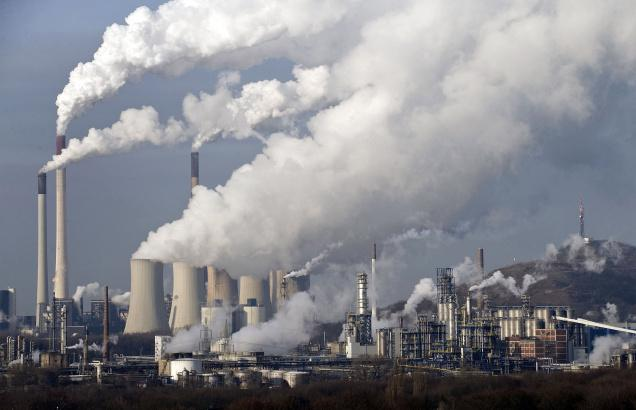
\includegraphics[width=1\linewidth]{pollution.jpg}
  \end{center}
\end{figure}
\begin{figure}[htpb]
  \begin{center}
	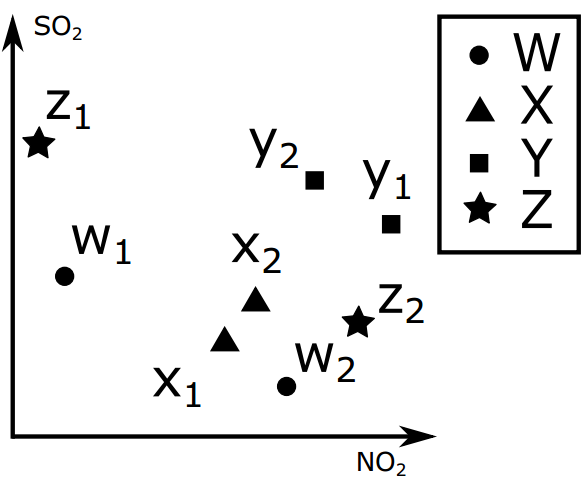
\includegraphics[width=0.75\linewidth]{coordinate.png}
  \end{center}
\end{figure}

\column{.58\textwidth} % Right column and width
\begin{table}[htbp]
\scriptsize
\begin{tabular}{|c|c|c|c|c|}
\hline Object&Instance&NO$_2$&SO$_2$& Probability\\
\hline
\multirow{2}{*}{W}
             &w$_1$   &10    &40    &0.5\\
             &w$_2$   &75    &10    &0.4\\\hline
\multirow{2}{*}{X}
             &x$_1$   &55    &20    &0.2\\
             &x$_2$   &65    &30    &0.2\\\hline
\multirow{2}{*}{Y}
             &y$_1$   &95    &60    &0.8\\
             &y$_2$   &80    &70    &0.2\\\hline
\multirow{2}{*}{Z}
             &z$_1$   & 5    &80    &0.5\\
             &z$_2$   &90    &25    &0.5\\
\hline
\end{tabular}
\end{table}
\tiny
\begin{align*}
P_{sky}(y_1)&=P(y_1)(1-P(w_1)-P(w_2))(1-P(x_1)-P(x_2))(1-P(z_2))\\
            &=0.024\\
P_{sky}(y_2)&=0.012\\
P_{sky}(Y)&= P_{sky}(y_1)+P_{sky}(y_2) = 0.036\\
P_{sky}(W)&= 0.9\\
P_{sky}(X)&= 0.4\\
P_{sky}(Z)&= 0.74\\
\end{align*}


\end{columns}
\end{frame}


%--------------Frame 5---------------------
\begin{frame}
\frametitle{Probabilistic Skylines}
%\begin{itemize}
%\item Lorem ipsum dolor sit amet, consectetur adipiscing elit
%\item Aliquam blandit faucibus nisi, sit amet dapibus enim tempus eu
%\item Nulla commodo, erat quis gravida posuere, elit lacus lobortis est, quis porttitor odio mauris at libero
%\item Nam cursus est eget velit posuere pellentesque
%\item Vestibulum faucibus velit a augue condimentum quis convallis nulla gravida
%\end{itemize}
\begin{block}{Probabilistic Skyline Problem}
For a set of uncertain objects $\mathbb{D}$ and a probability threshold $T_p$, the probabilistic skyline $pSL(\mathbb{D}, T_p)$, is the set of all objects whose skyline probabilities are at least $T_p$, $pSL(\mathbb{D}, T_p) = \{U \in \mathbb{D} | P_{sky}(U) \geq T_p\}$.
\end{block}
The discrete model:
\begin{align*}
P_{sky}(U) = \sum\limits_{u_i\in U} P_{sky}(u_i)= \sum\limits_{u_i\in U} (P(u_i)\times\prod\limits_{V\in\mathbb{D},V\neq U}(1-\sum\limits_{v_j\in V,v_j\prec u_i}P(v_j)))
\end{align*}
The continuous model:
\begin{align*}
P_{sky}(u_i) = \int_{U}Uf(u)\times\prod\limits_{V\in\mathbb{D},V\neq U}(1-\int_{V}Vf(v)1(v\prec u)\,dv)\,du
\end{align*}

\end{frame}

%--------------Frame 6---------------------
\begin{frame}
\frametitle{What is MapReduce?}
\begin{columns}[c]
\column{.42\textwidth} % Left column and width
\begin{figure}[htpb]
  \begin{center}
	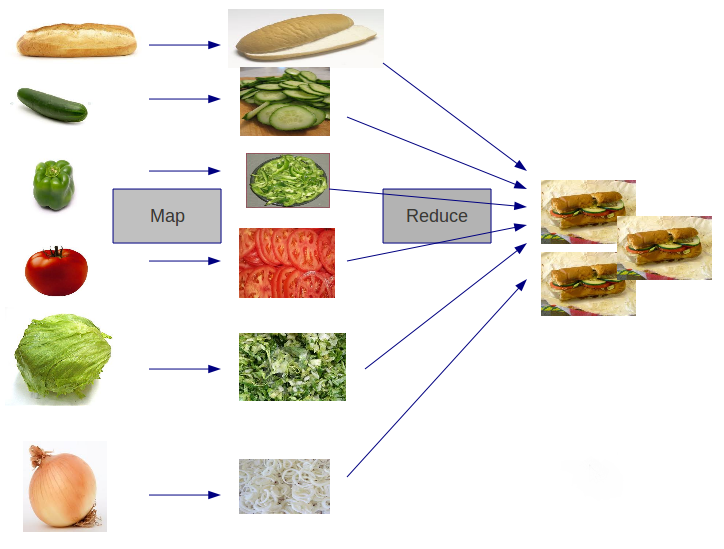
\includegraphics[width=\linewidth]{mapreduce1.png}
  \end{center}
\end{figure}

\column{.42\textwidth} % Right column and width
\begin{figure}[htpb]
  \begin{center}
	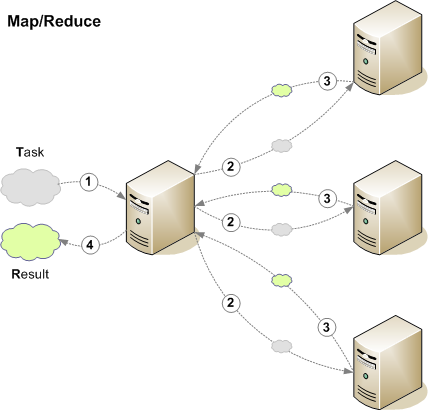
\includegraphics[width=\linewidth]{mapreduce2.png}
  \end{center}
\end{figure}
\end{columns}
\end{frame}

%--------------Frame 7---------------------
\begin{frame}
\frametitle{PSMR: The State-of-the-art Algorithm}
\begin{columns}[c] % The "c" option specifies centered vertical alignment while the "t" option is used for top vertical alignment

\column{.4\textwidth} % Left column and width
\begin{figure}[htpb]
  \begin{center}
	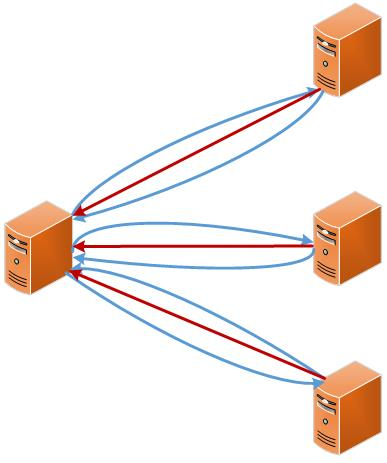
\includegraphics[width=0.9\linewidth]{psmr.jpg}
  \end{center}
\end{figure}

\column{.6\textwidth} % Right column and width
\begin{enumerate}
\item local computing candidate sets.
\item merge candidate sets, broadcast and local computing, reduce probabilities.
\end{enumerate}

\end{columns}
\end{frame}

%\section{Second Section}

%--------------Frame 8--------------------
\begin{frame}
\frametitle{Early Pruning Techniques}
%\begin{table}
%\begin{tabular}{l l l}
%\toprule
%\textbf{Treatments} & \textbf{Response 1} & \textbf{Response 2}\\
%\midrule
%Treatment 1 & 0.0003262 & 0.562 \\
%Treatment 2 & 0.0015681 & 0.910 \\
%Treatment 3 & 0.0009271 & 0.296 \\
%\bottomrule
%\end{tabular}
%\caption{Table caption}
%\end{table}

\begin{lemma}[Zero-probability Filtering]
$P_{sky}(U)=\sum\limits_{u_i\in U} P(u_i)\times\prod\limits_{V\in\mathbb{D},V\neq U}(1-\sum\limits_{v_j\in V,v_j\prec u_i}P(v_j))$\\
delete $u_i$ if $\prod\limits_{V\in\mathbb{D},V\neq U}(1-\sum\limits_{v_j\in V,v_j\prec u_i}P(v_j)) = 0$.
\end{lemma}

\begin{columns}[c] % The "c" option specifies centered vertical alignment while the "t" option is used for top vertical alignment
\column{.4\textwidth} % Left column and width
\begin{figure}[htpb]
  \begin{center}
	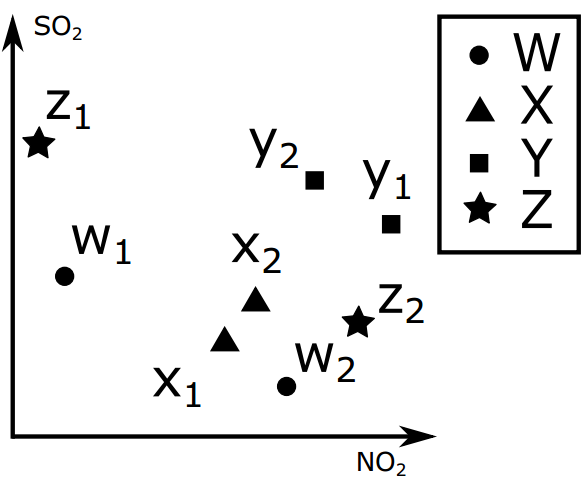
\includegraphics[width=\linewidth]{coordinate.png}
  \end{center}
\end{figure}

\column{.55\textwidth} % Right column and width
\begin{example}[Zero-probability Filtering]
we can see, $x_1$ dominate $y_1$, if $P(x_1)=1$, then $P_{sky}(y_1)=0$
\end{example}
\end{columns}
\end{frame}

%--------------Frame 9---------------------
\begin{frame}
\frametitle{Early Pruning Techniques}

\begin{lemma}[Upper-bound Filtering]
$\beta(U, \mathbb{S}, R(u_i))=\frac{\prod\limits_{V\in\mathbb{S}}(1-\sum\limits_{v_j\in V,v_j\prec R(u_i).min}P(v_j))}{1- \sum\limits_{v_k\in U,v_k\prec R(u_k).min}P(v_j) }$\\

$up(u_i, U, \mathbb{S}, R(u_i)) = P(u_i)\times \beta(U, \mathbb{S}, R(u_i))$.
\end{lemma}

\begin{columns}[c] % The "c" option specifies centered vertical alignment while the "t" option is used for top vertical alignment
\column{.4\textwidth} % Left column and width
\begin{figure}[htpb]
  \begin{center}
	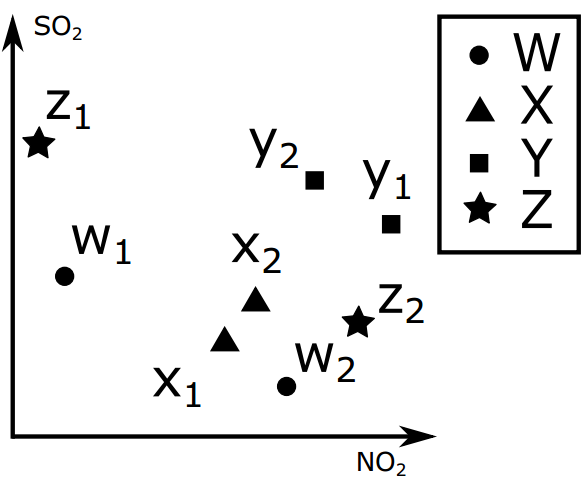
\includegraphics[width=\linewidth]{coordinate.png}
  \end{center}
\end{figure}

\column{.6\textwidth} % Right column and width
\begin{example}[Upper-bound Filtering]
\tiny
\begin{align*}
P_{sky}(y_1)&=P(y_1)(1-P(w_1)-P(w_2))(1-P(x_1)-P(x_2))(1-P(z_2))\\
            &\leq P(y_1)(1-P(w_1))=0.4\\
P_{sky}(y_2)&\leq0.1\\
P_{sky}(Y)& = P_{sky}(y_1) + P_{sky}(y_2) \leq 0.5 < T_p\\
\end{align*}
\end{example}
\end{columns}

\end{frame}

%--------------Frame 10--------------------
\begin{frame}
\frametitle{Early Pruning Techniques}
\begin{lemma}[Dominance-Power Filtering]
$DP(v_j)=\prod\limits_{1}^{d}(b(k)-v_j(k))=0, b(k) = max\{v_1(k),\cdots,v_n(k)\}$.\\
$DP(V) = \sum_{v_j\in V}(P(v_j)\times DP(v_j))$.\\
$\mathbb{F}$ is top$K$ $DP$ set, $\sum\limits_{u_i\in U} P(u_i)\times\prod\limits_{V\in\mathbb{F},V\neq U}(1-\sum\limits_{v_j\in V,v_j\prec u_i}P(v_j))<T_p$, $U$ is not a probabilistic skyline Object.\\
\end{lemma}

\begin{columns}[c] % The "c" option specifies centered vertical alignment while the "t" option is used for top vertical alignment
\column{.38\textwidth} % Left column and width
\begin{figure}[htpb]
  \begin{center}
	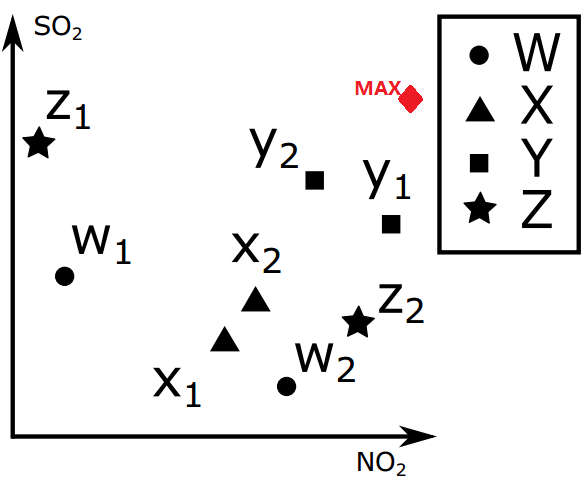
\includegraphics[width=\linewidth]{coordinate2.png}
  \end{center}
\end{figure}

\column{.55\textwidth} % Right column and width
\begin{example}[Dominance-Power Filtering]
\footnotesize
\begin{align*}
DP(y_1)&=(100-95)(100-60)=200\\
DP(y_2)&=(100-80)(100-70)=600\\
DP(Y)& = P(y_1)*DP(y_1) + P(y_2)*DP(y_2) \\
     &= 0.8*200+0.2*600 = 280\\
\end{align*}
\end{example}
\end{columns}
\end{frame}


%--------------Frame 11---------------------
%\begin{frame}[fragile] % Need to use the fragile option when verbatim is used in the slide
%\frametitle{Verbatim}
%\begin{example}[Theorem Slide Code]
%\begin{verbatim}
%\begin{frame}
%\frametitle{Theorem}
%\begin{theorem}[Mass--energy equivalence]
%$E = mc^2$
%\end{theorem}
%\end{frame}\end{verbatim}
%\end{example}
%\end{frame}
\begin{frame}
\frametitle{PSQtree for Pruning}
\begin{figure}[htpb]
  \begin{center}
	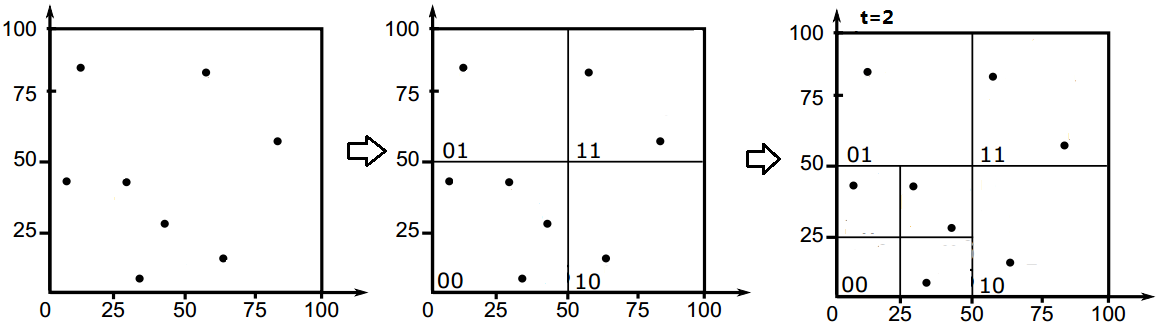
\includegraphics[width=\linewidth]{PSQtree.png}
  \end{center}
\end{figure}
\begin{columns}[t]
\column{.6\textwidth}
\begin{itemize}
\item generate PSQtree
\item traverse PSQtree for computing $P_{sky}(node.min)$
\item zero-probability filtering
\item upper-bound filtering
\item partitioning objects by PSQtree(weakly dominate)
\end{itemize}

\column{.35\textwidth}
\begin{figure}[htpb]
  \begin{center}
	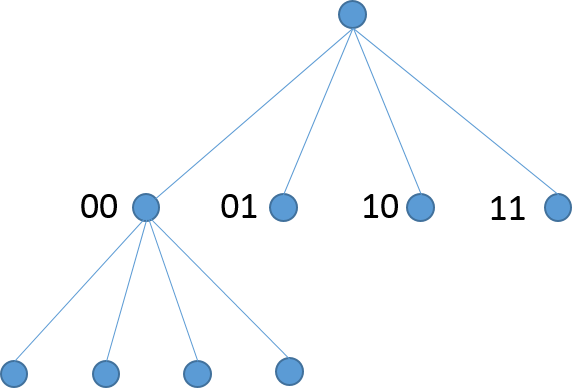
\includegraphics[width=\linewidth]{tree.png}
  \end{center}
\end{figure}
\end{columns}

\end{frame}


%--------------Frame 12---------------------
\begin{frame}
\frametitle{MapReduce Algorithms with PSQtree}
\begin{figure}[htpb]
  \begin{center}
	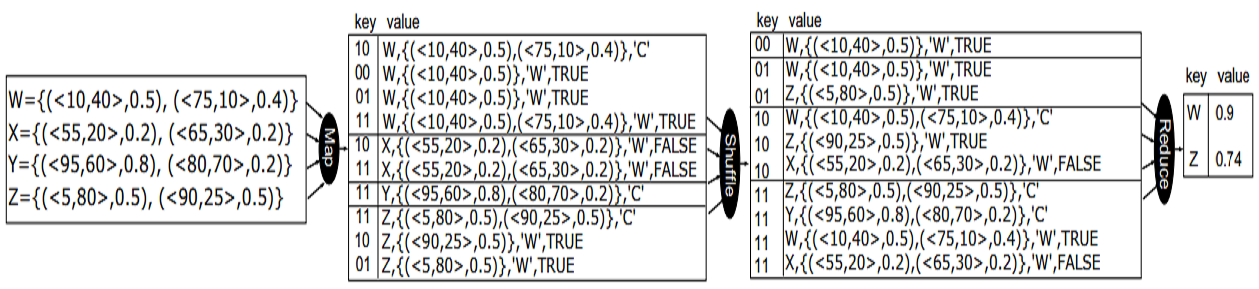
\includegraphics[width=\linewidth]{PS-QPFC-MR.png}
  \end{center}
\end{figure}

\begin{columns}[c] % The "c" option specifies centered vertical alignment while the "t" option is used for top vertical alignment
\column{.3\textwidth} % Left column and width
\begin{figure}[htpb]
  \begin{center}
	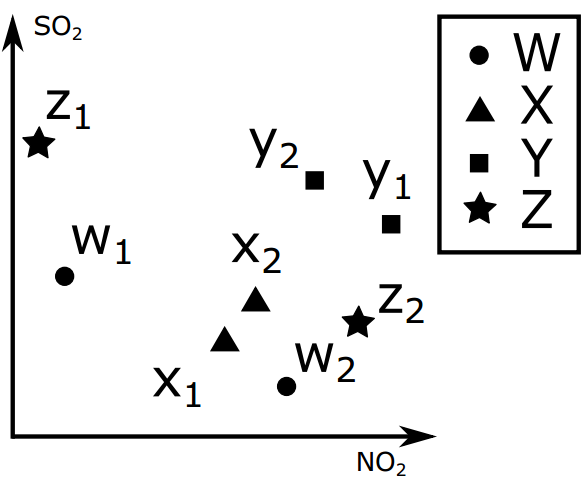
\includegraphics[width=\linewidth]{coordinate.png}
  \end{center}
\end{figure}

\column{.7\textwidth} % Right column and width
\begin{example}[PS-QPF-MR]
\tiny
\begin{itemize}
\item $T_p$ = 0.5, map function is called with an uncertain object.\\
\item for $X$, upper bound $node(10).P_{min} �� P (x1) + node(10).P_{min} �� P (x2) = 0.4 < T_p = 0.5$.\\
$X$ is not a skyline candidate. \\
\item every instance of $X$, emit the key-value pairs $\langle10, (\{(\langle55, 20\rangle, 0.2), (\langle65,
30\rangle, 0.2)\},��W��, False)\rangle and \langle11,(\{(\langle55, 20\rangle, 0.2),$\\$(\langle65, 30\rangle,
0.2)\},��W��, False)\rangle$since node(10) weakly dominates node(10) and node(11)
\end{itemize}
\end{example}
\end{columns}

\end{frame}




%--------------Frame 13--------------------
\begin{frame} % Need to use the fragile option when verbatim is used in the slide
\frametitle{Experiments}
\begin{itemize}
\item 50 machines with Intel i3 3.3GHz CPU and 4GB, Linux
\item 200 machines with Intel Xeon 2.5GHz CPU and 3.75GB, Amazon EC2
\item Java 1.6, Hadoop 1.2.1
\end{itemize}
\begin{table}[htbp]
\scriptsize
\begin{tabular}{|c|l|}
\hline Algorithm& Description  \\
\hline
PS-QP-MR&The algorithm with quadtree partitioning\\
\hline
PS-QPF-MR&The algorithm with quadtree partitioning and filtering\\
\hline
PS-BR-MR&The algorithm with random partitioning \\
\hline
PS-BRF-MR&The algorithm with random partitioning and filtering\\
\hline
PSMR& The state-of-the-art algorithm \\
\hline
\end{tabular}
\end{table}
\begin{table}[htbp]
\scriptsize
\begin{tabular}{|c|c|p{3cm}|}
\hline Parameter& Range &  Default \\
\hline
No. of samples($\mathbb{S}$)&1000$\sim$10,000 &1000 for PS-QPF-MR 2000 for PS-QP-MR 10000 for PS-BRF-MR \\
\hline
No. of dominating objects($\mathbb{F}$) &1000$\sim$10,000 &100 for PS-QPF-MR 1000 for PS-BRF-MR \\
\hline
No. of objects($\mathbb{D}$)&$10^5\sim10^8$ & $10^7$ \\
\hline
No. of dimensions($d$)&2 $\sim$ 8 &4\\
\hline
Probability threshold ($T_p$) & 0.1$\sim$0.6 &0.3 \\
\hline
No. of inst. per object($\ell$)&1 $\sim$ 400 &40 \\
\hline
No. of machines ($t$) &10$\sim$200 &25\\
\hline
\end{tabular}
\end{table}

\end{frame}

%--------------Frame 14--------------------
\begin{frame} % Need to use the fragile option when verbatim is used in the slide
\frametitle{Experiments}
\begin{figure}[htpb]
  \begin{center}
	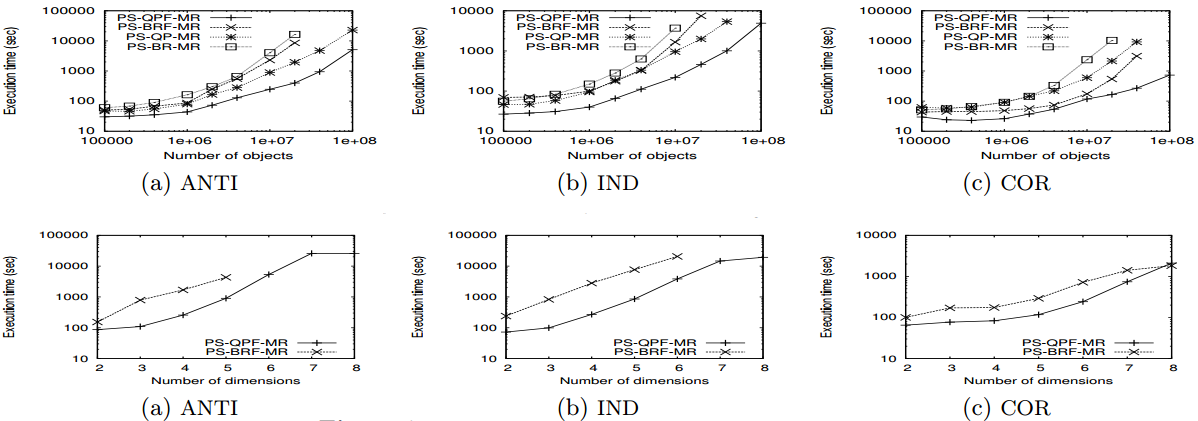
\includegraphics[width=\linewidth]{algorithm-comparison.png}
  \end{center}
\end{figure}
\end{frame}


%--------------Frame 15--------------------
\begin{frame} % Need to use the fragile option when verbatim is used in the slide
\frametitle{Experiments}
\begin{figure}[htpb]
  \begin{center}
	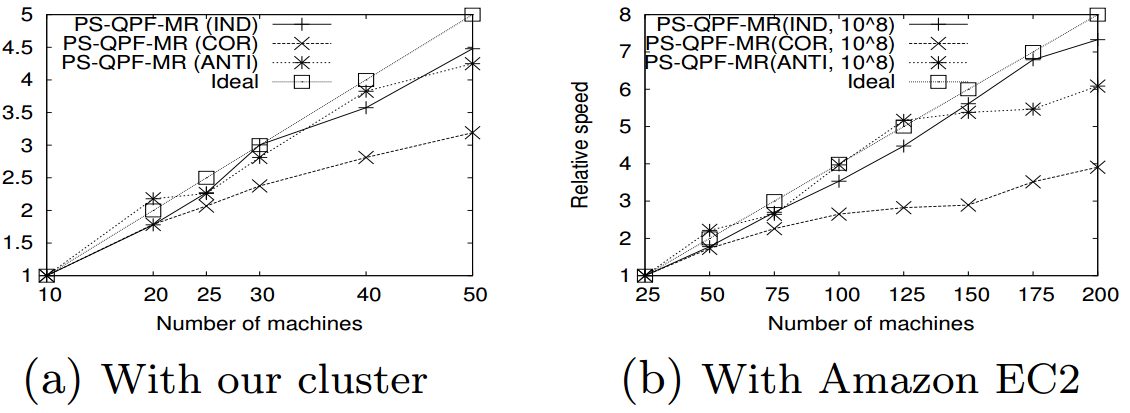
\includegraphics[width=0.9\linewidth]{cluster-comparison.png}
  \end{center}
\end{figure}

\begin{figure}[htpb]
  \begin{center}
	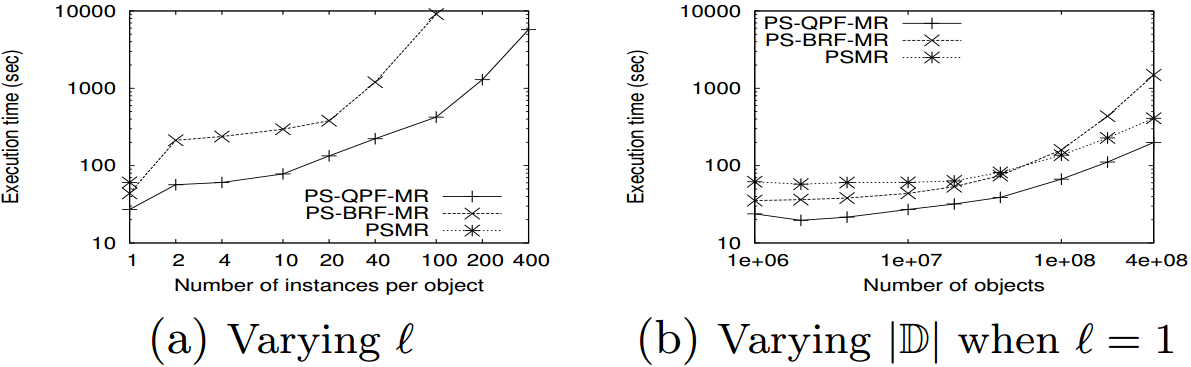
\includegraphics[width=0.9\linewidth]{algorithm-comparison2.png}
  \end{center}
\end{figure}
\end{frame}

%--------------Frame 16--------------------
\begin{frame} % Need to use the fragile option when verbatim is used in the slide
\frametitle{Conclusion}
\begin{itemize}
\item probabilistic skyline query for both discrete and continuous models
\item zero-probability, the upper-bound, and dominance power filtering techniques
\item using a PSQtree to distribute the instances of objects effectively
\item a single MapReduce phase algorithm PS-QPF-MR and grouping techniques for optimization
\end{itemize}
\end{frame}

%\begin{frame}
%\frametitle{References}
%\footnotesize{
%\begin{thebibliography}{99} % Beamer does not support BibTeX so references must be inserted manually as below
%\bibitem[Smith, 2012]{p1} John Smith (2012)
%\newblock Title of the publication
%\newblock \emph{Journal Name} 12(3), 45 -- 678.
%\end{thebibliography}
%}
%\end{frame}


%--------------Frame 17--------------------
\begin{frame}
\frametitle{The End}
\Huge{\centerline{Q \& A}}
\end{frame}

%----------------------------------------------------------------------------------------

\end{document}
